\documentclass[dvipdfmx]{standalone}

\usepackage{adjustbox}      % \begin{adjustbox}
\usepackage[ruled, vlined]{algorithm2e}    % \begin{algorithm2e}
\usepackage{amsmath}        % \begin{align*}
\usepackage{amssymb}        % \mathbb{A}
\usepackage{amsthm}         % \newtheorem
\usepackage{bm,bbm}         % \bm{A}, \bbm{1}
\usepackage{booktabs}       % \toprule, \midrule, \bottomrule
\usepackage{enumitem}       % \begin{enumerate}[label=(\alph*)]
\usepackage{hyperref}       % \href{URL}{text}
\usepackage{ifthen}         % \ifthenelse
\usepackage{lipsum}         % \lipsum
\usepackage{makecell}       % \makecell{L1\L2}
\usepackage{mathrsfs}       % \mathscr{A}
\usepackage{mathtools}      % \mathrlap
\usepackage{multirow}       % \multirow
\usepackage{optidef}        % \begin{mini*}{x}{f(x)}{}{}
\usepackage{orcidlink}      % \orcidlink
\usepackage{physics}        % \qty, \norm, \abs
\usepackage{subcaption}     % \captionsetup
\usepackage{subfiles}       % \subfile{file}
\usepackage{thm-restate}    % \begin{restatable}{theorem}{thm}
\usepackage{tikz}           % \begin{tikzpicture}
\usepackage{xparse}         % \NewDocumentCommand

\definecolor{cA}{HTML}{0072BD}
\definecolor{cB}{HTML}{EDB120}
\definecolor{cC}{HTML}{77AC30}
\definecolor{cD}{HTML}{D95319}
\definecolor{cE}{HTML}{7E2F8E}
\newcommand{\cAText}[1]{\textcolor{cA}{#1}}
\newcommand{\cBText}[1]{\textcolor{cB}{#1}}
\newcommand{\cCText}[1]{\textcolor{cC}{#1}}
\newcommand{\cDText}[1]{\textcolor{cD}{#1}}
\newcommand{\cEText}[1]{\textcolor{cE}{#1}}

\usetikzlibrary{
  arrows.meta,
  calc,
  fit,
  positioning,
  shapes.geometric,
}

\begin{document}
\begin{tikzpicture}
  \node[cA,font=\bfseries] (A) at (0,0) {Graph Drawing};
  \node[cB] (B) at (-3.0,-1) {Discrete Based};
  \node[align=left,anchor=north west] (B1) at ($(B)+(-2.0,-0.6-0.0)$) {\cBText{BFS layout}\\\small{\quad - for tree graph}};
  \node[align=left,anchor=north west] (B2) at ($(B)+(-2.0,-0.6-1.0)$) {\cBText{Planar layout}\\\small{\quad - for planar graph}\\\scriptsize{\quad - \cite{tutteHowDrawGraph1963}}\\\scriptsize{\quad - \cite{chrobakLineartimeAlgorithmDrawing1995}}};
  \node[align=left,anchor=north west] (B3) at ($(B)+(-2.0,-0.6-3.0)$) {\cBText{Layered graph drawing}\\\small{\quad - for DAG}\\\scriptsize{\quad - \cite{sugiyamaMethodsVisualUnderstanding1981}}};
  \node[align=left,anchor=north west] (B4) at ($(B)+(-2.0,-0.6-4.5)$) {\cBText{Spectral layout~}\\\small{\quad - eigenvector of Laplacian}};
  \node[draw=cB, thick,fit={(B1) (B2) (B3) (B4)}, inner sep=5pt] (BBox) {};

  \node[cC,font=\bfseries] (C) at (+4.5,-1) {Continuous Based};
  \node[cC] (C1) at ($(C)+(-2.5,-1)$) {Kamada--Kawai (KK)};
  \node at ($(C1)+(0,-1.0)$) {
    \begin{minipage}{4cm}
      \begin{gather*}
        \mathrm{minimize}\\
        \sum_{i < j} \frac{k_{i,j}}{2} (d_{i,j}-l_{i,j})^2
      \end{gather*}
    \end{minipage}
  };
  \node[cC,font=\bfseries] (C2) at ($(C)+(+2.5,-1)$) {Fruchterman--Reingold (FR)};
  \node at ($(C2)+(0,-1.0)$) {
    \begin{minipage}{4cm}
      \begin{gather*}
        \mathrm{minimize}\\
        \sum_{i<j} \qty(\frac{a_{i,j} d_{i,j}^3}{3k} - k^2\log{d_{i,j}})
      \end{gather*}
    \end{minipage}
  };

  \node[align=center] (C3) at ($(C)+(0.5,-4.3)$) {
  \scriptsize{$d_{i,j}$: distance between nodes $v_i,v_j$ \;/\; $l_{i,j}$: optimal distance \;/\; $k,a_{i,j}$: constant}
  };

  \node (C01) at ($(C)+(-3.5,-5.5)$) {
    
\includegraphics[width=1cm]{networkxLogo.png}
  };
  \node (C02) at ($(C)+(-2.5,-5.5)$) {
    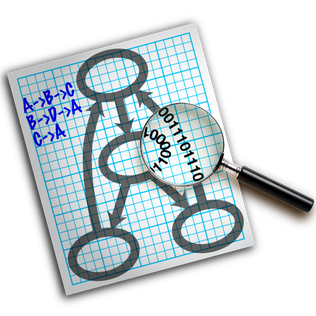
\includegraphics[width=1cm]{GraphvizLogo.png}
  };
  \node[anchor=west] (C03) at ($(C)+(-2,-5.5)$) {
    NetworkX and Graphviz support KK and FR
  };
  \node[draw=cC, thick,fit={(C01) (C02) (C03)}, inner sep=5pt] (CBox) {};

  \draw[thick,-{Stealth[length=2mm]}] (A) |- ($(A)!0.5!(B)$) -| (B);
  \draw[thick,-{Stealth[length=2mm]}] (A) |- ($(A)!0.5!(C)$) -| (C);
  \draw[thick,-{Stealth[length=2mm]}] (C) |- ($(C)!0.5!(C1)$) -| (C1);
  \draw[thick,-{Stealth[length=2mm]}] (C) |- ($(C)!0.5!(C2)$) -| (C2);
\end{tikzpicture}
\end{document}